\subsection{Measurement methods}
\paragraph{Task 1:} The LiF-crystal is examined with the radiation set to an accelearting voltage of \(U_a=\qty{35}{\kilo\V}\) by automatically turning the crystal from \(\qtyrange{3}{22}{\degree}\) in steps of \(\Delta \vartheta=\ang{0.2}\) and measuring the resulting intensity of the reflected/scattered radiation with an exposure time of \(t=\qty{5}{\s}\). 

\paragraph{Task 2:} 
With the plot given by the first task, one can determine the \(K_\alpha\) and \(K_\beta\) lines of first and second order, and examine them a bit more in detail by only choosing the individual angle-range of said lines and scanning them with \(\Delta \vartheta=\ang{0.1}\) and \(t=\qty{20}{\s}\).

\paragraph{Task 3:} The count rate/intensity is recorded with constant \(\vartheta=\ang{7.5}\) as a function of \(U_a\), therefore one varies \(U_a\) between \(\qtyrange{20}{35}{\kilo\volt}\) in steps of \(\qty{1}{\kilo\volt}\), each time with \(t=\qty{20}{\s}\).

\paragraph{Task 4:} Same procedure as in task 1 is performed, this time with the NaCl-crystal, the only difference is an angle-range of \(\qtyrange{3}{18}{\degree}\).
\vfill
\subsection{Lab protocol / data sheet}
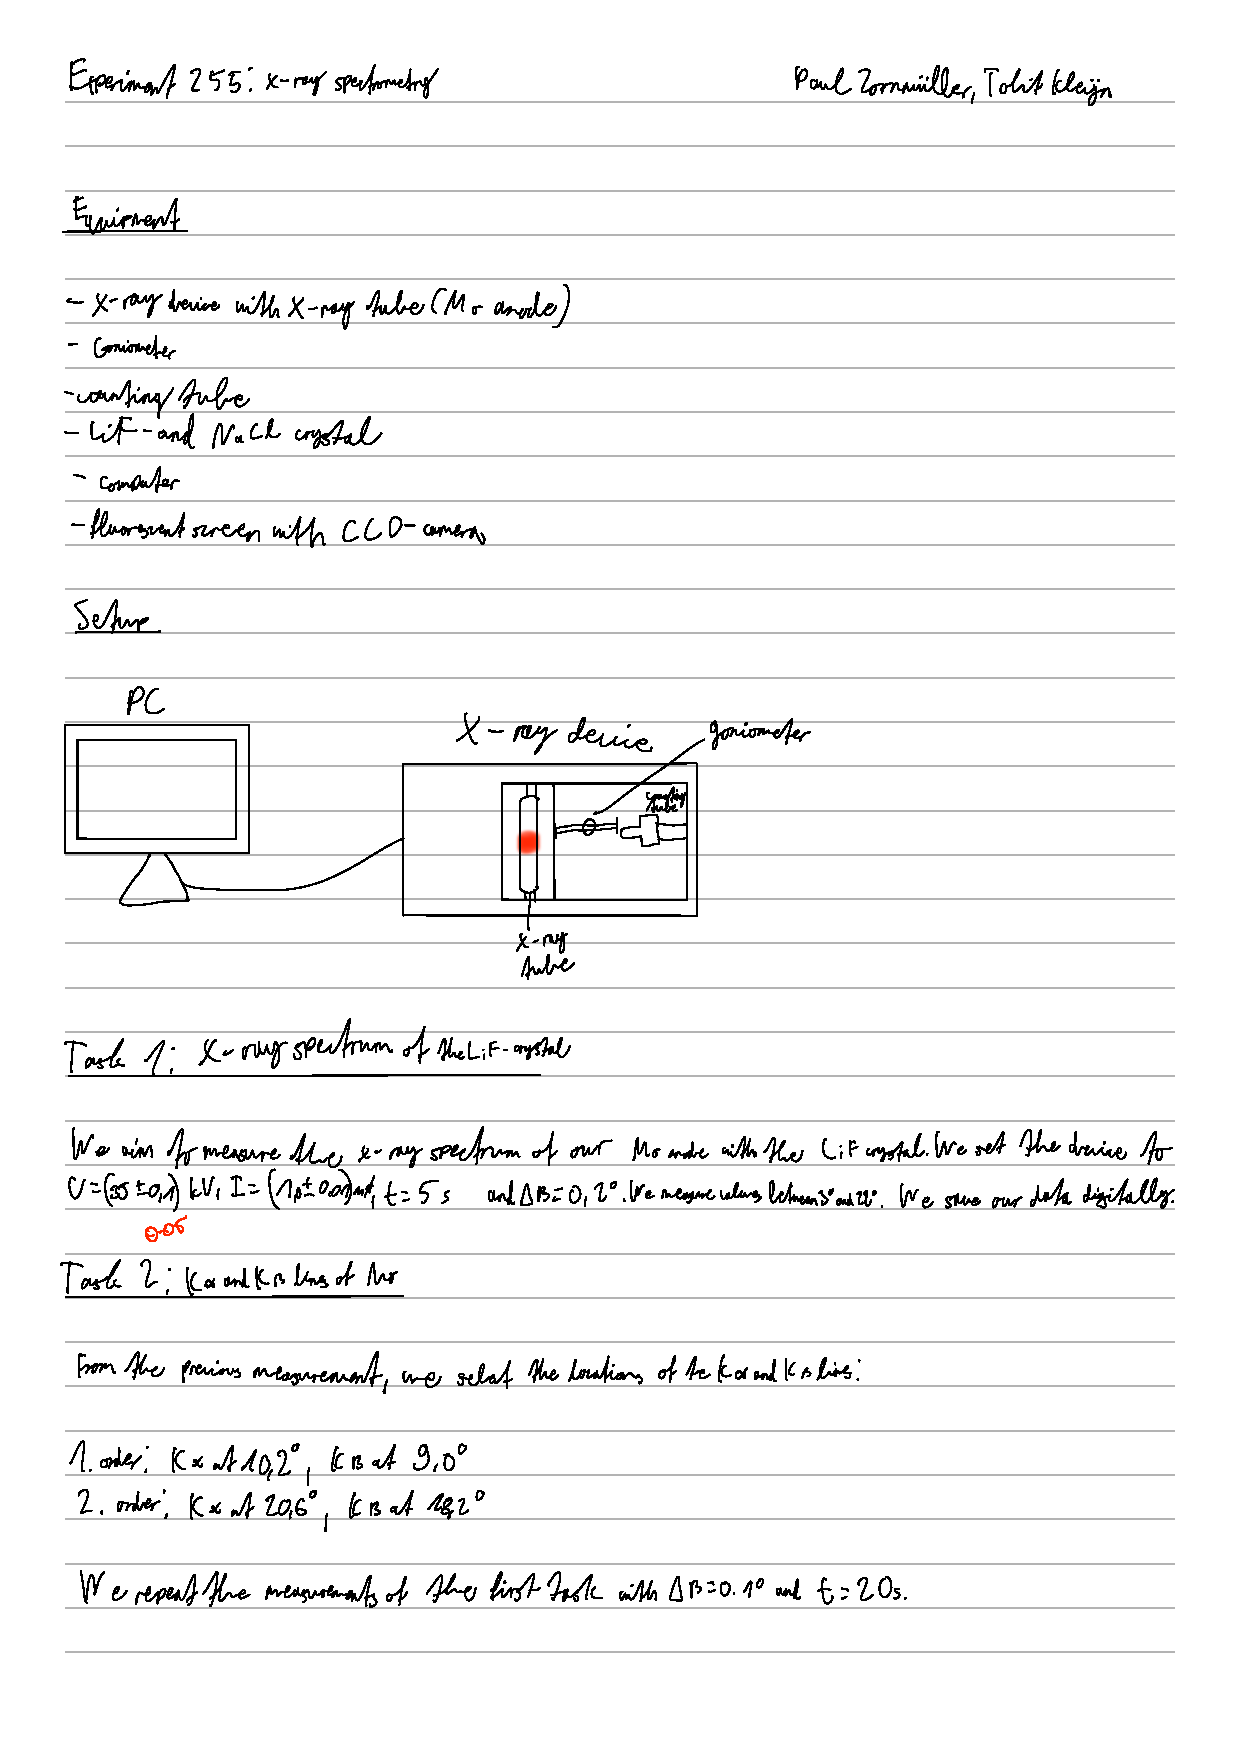
\includepdf[pages=-]{./images/255}
